\chapter{Resultados y pruebas}
\label{chap:results}
\vspace{0.5cm}

%%%%%%%%%%%%%%%%%%%%%%%%%%%%%%%%%%%%%%%%%%%%%%%%%%%%%%%%%%%%%%%%%%%%%%%%%%%%%%%%
% Objetivo: Exponer los resultados objetivos del sistema                       %
%%%%%%%%%%%%%%%%%%%%%%%%%%%%%%%%%%%%%%%%%%%%%%%%%%%%%%%%%%%%%%%%%%%%%%%%%%%%%%%%

 
\lettrine{E}{n} este capítulo se expondrán los resultados y el funcionamiento de los módulos desarrollados en este trabajo mediante tres aplicaciones de ejemplo.
\section{Ejemplos de uso}
Para probar el correcto funcionamiento de los módulos de interacción, a parte de los ejemplos de desarrollo que se comentaron en el capítulo \ref{sec:InteractionLibraries}, se desarrollaron tres aplicaciones para ROBOBO utilizando las librerías de interacción diseñadas y desarrolladas en este proyecto.

\subsection{Simón dice musical}
\label{subsec:simon-musical}
El primero de los ejemplos desarrollados es un juego educativo musical, similar al juego Simón dice, en el que los participantes deben repetir una secuencia de colores que se va ampliando en cada iteración de la partida, pero utilizando notas musicales. El objetivo final de este juego es que el usuario consiga asociar los tonos escuchados con la nota musical correspondiente, además de ejercitar la memoria.
En este ejemplo se han utilizado los siguientes módulos:

\begin{itemize}
	\item \textbf{SoundDispatcherModule:} Necesario para el funcionamiento de los módulos de sonido
	\item \textbf{PitchDetectionModule:} Usado indirectamente por el NoteDetectionModule
	\item \textbf{NoteDetectionModule:} Utilizado a la hora de detectar las notas musicales producidas por el usuario.
	\item \textbf{ClapDetectionModule:} Se utiliza para iniciar el juego, una primera palmada prepara al robot y la segunda inicia el juego.
	\item \textbf{EmotionSoundModule:} Diferentes sonidos son reproducidos en función del resultado del juego.
	\item \textbf{NoteGeneratorModule:} Se emplea para generar los diferentes tonos que debe reconocer el jugador.
	\item \textbf{SpeechProductionModule:} Se usa para dar información al usuario y dar una mayor sensación de interacción con el robot
\end{itemize}

Además de los módulos creados en este trabajo, se emplean varios módulos que provee el ROBOBO! Framework:

\begin{itemize}
	\item \textbf{EmotionModule:} Provee la cara del robot, con la posibilidad de cambiar sus expresiones, es la interfaz gráfica que se le muestra al usuario.
	\item \textbf{DefaultMovementModule:} Permite el uso de la plataforma robótica de forma simple, permitiendo el movimiento del robot.
	\item \textbf{IRobInterfaceModule:} Proporciona un método para obtener la clase IRob, que se emplea para un control más avanzado del Rob, por ejemplo, para utilizar los leds de la base.
\end{itemize}


\begin{figure}
	\centering
	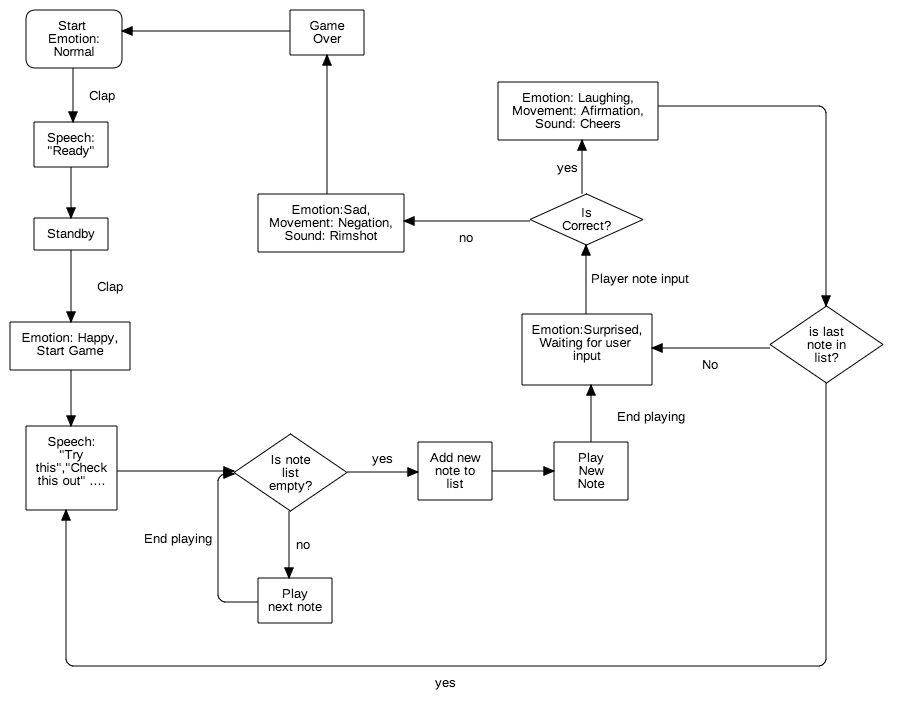
\includegraphics[width=1.1\linewidth]{imagenes/simon_flowchart.png}
	\caption{Diagrama de flujo del ejemplo musical}
	\label{fig:simon-flowchart}
\end{figure} 


El robot comienza la partida desactivado (figura \ref{fig:simon-normal}), el jugador inicia la partida dando una palmada, momento en el que el robot pronunciará a través del modulo de voz \enquote{Ready}(\ref{fig:simon-smile} , una segunda palmada comenzará la partida en si, el robot dirá una frase retando al usuario, por ejemplo \enquote{follow me if you can}, y procederá a reproducir un tono musical. En el momento en el que termine el tono, cambiará la cara (figura \ref{fig:simon-surprised} dando a entender que está escuchando al usuario, en el momento en el que el jugador termine de producir la nota se comprueba si corresponde al tono original, si coincide el robot realizará una pequeña celebración y volverá a producir tonos, añadiendo uno más a los reproducidos anteriormente. En caso de que el jugador falle, el robot pondrá cara de disgusto (figura \ref{fig:simon-sad}), producirá un sonido de abucheo y volverá al estado inicial, esperando a una palmada para iniciar el juego. Este proceso puede observarse en el diagrama de flujo que se muestra en la figura \ref{fig:simon-flowchart}.

\begin{figure}
	\centering
	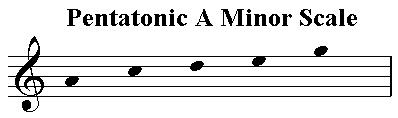
\includegraphics[width=0.6\linewidth]{imagenes/pentatonic-scale-a-minor.jpg}
	\caption{Escala pentatonica menor de La}
	\label{fig:pentatonic-scale}
\end{figure} 

\begin{figure}[h]
\centering
\begin{minipage}{0.45\textwidth}
\centering
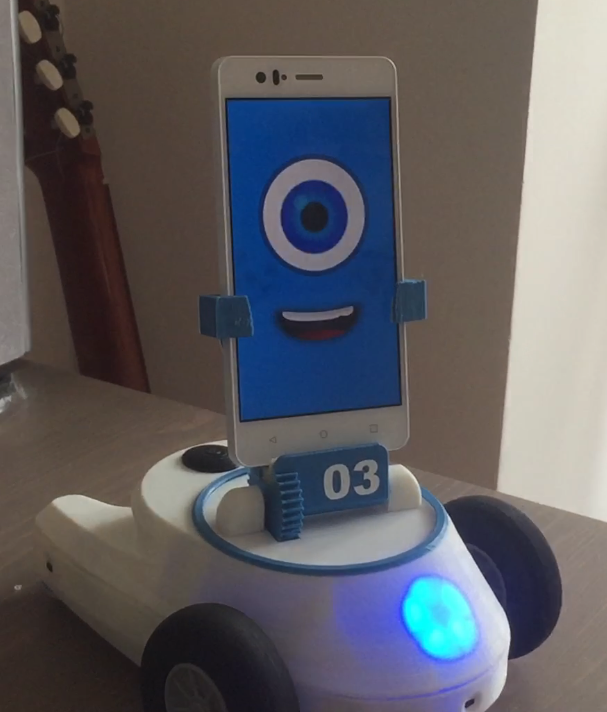
\includegraphics[width=1\linewidth]{imagenes/simon_normal.png}
\caption{ROBOBO Desactivado}
\label{fig:simon-normal}

\end{minipage}\hfill
\begin{minipage}{0.45\textwidth}
\centering
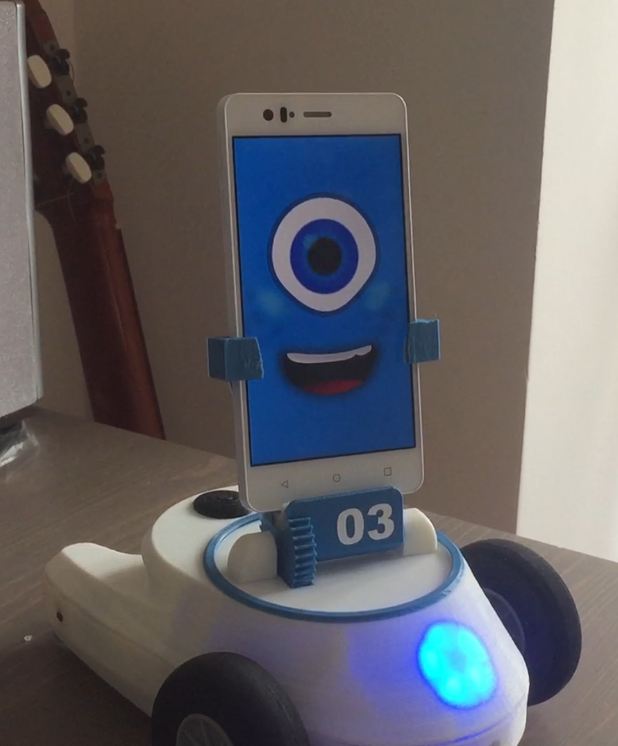
\includegraphics[width=1\linewidth]{imagenes/simon_smile.png}

\caption{ROBOBO en Standby}
\label{fig:simon-smile}

\end{minipage}
\end{figure}

\begin{figure}[h]
\centering
\begin{minipage}{0.45\textwidth}
\centering
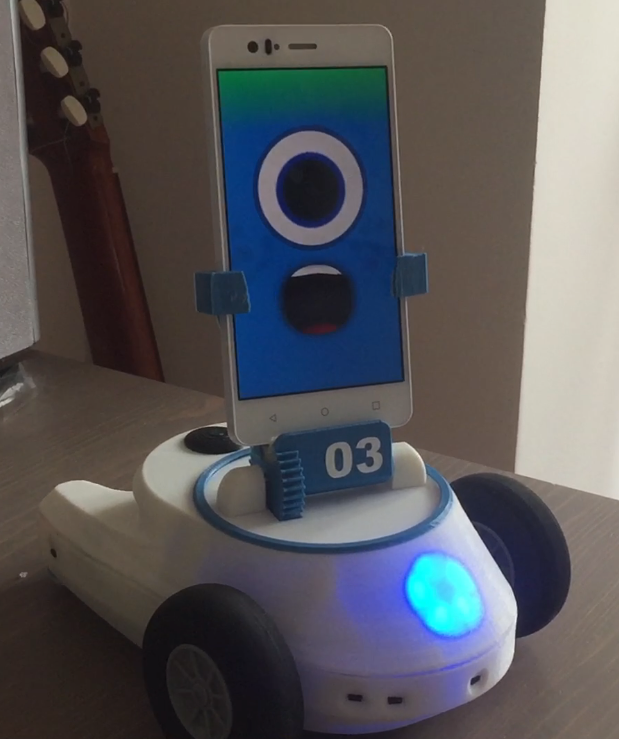
\includegraphics[width=1\linewidth]{imagenes/simon_surprised.png}
\caption{ROBOBO escuchando al usuario}
\label{fig:simon-surprised}

\end{minipage}\hfill
\begin{minipage}{0.45\textwidth}
\centering
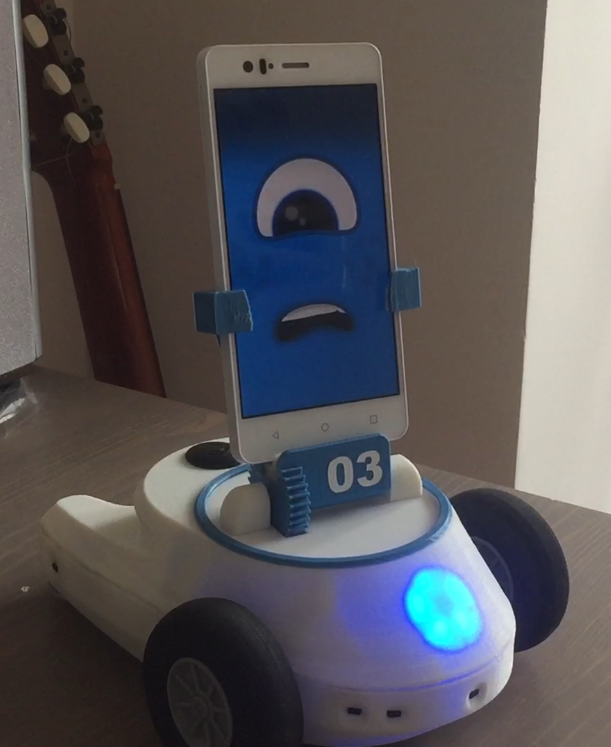
\includegraphics[width=1\linewidth]{imagenes/simon_sad.png}

\caption{ROBOBO tras fallar la nota}
\label{fig:simon-sad}

\end{minipage}
\end{figure}


En este ejemplo se pueden ver en funcionamiento múltiples módulos de interacción, por ejemplo a continuación puede verse el código empleado para iniciar la partida, que hace uso del listener \textit{OnClap} que proporciona el \textit{ClapDetectionModule}.

\vspace{5mm} %5mm vertical space

\begin{lstlisting}[language=Java][frame=single]
 @Override
    public void onClap(double time) {
        if ((ready)&&(!playing)){
            Log.d(TAG,"PLAYING");
            playing = true;
            startGame();
        }
        if ((!ready)&&(!playing)){
            Log.d(TAG,"READY");
            ready = true;
            emotionModule.setCurrentEmotion(Emotion.SMYLING);
            speechModule.sayText("Ready",0);
        }
    }

\end{lstlisting}

\vspace{5mm} %5mm vertical space

El siguiente fragmento de código es la implementación del listener \textit{onNoteEnd} del módulo \textit{NoteDetectionModule}, que es usado a la hora de detectar las notas que el jugador hace sonar. Para evitar falsos positivos, solo se tienen en cuenta las notas cuya duración supera los 200 milisegundos.

 \vspace{5mm} %5mm vertical space 
 
\begin{lstlisting}[language=Java][frame=single]
@Override
    public void onNoteEnd(com.mytechia.robobo.framework.hri.sound.noteDetection.Note note, long time) {

        Log.d(TAG, "NOTEEND!!!!!!! Playing: "+playing+" playingnotes "+playingnotes+" listening "+listening);

        if ((time>200)&&(playing)&&(!playingnotes)&&(listening)) {
            try {
                Log.d(TAG,"CheckResult");
                boolean checkresult = checkNote(convertNote(note));
                if (!checkresult){
                    Log.d(TAG,"GameOver");
                    gameOver();
                }
            }catch (NoSuchElementException e){
                Log.d(TAG,"EndList");
                listening = false;
                movTask = new AsienteClass();
                timermovement.schedule(movTask,0);
            }
        }
    }
\end{lstlisting}

\vspace{5mm} %5mm vertical space

También se ha implementado el listener de final de reproducción de secuencia \textit{onNoteSequenceEnd} en el que se crea la lista de notas a comprobar y se indica al sistema que debe comenzar a escuchar.

\vspace{5mm} %5mm vertical space

\begin{lstlisting}[language=Java][frame=single]
    @Override
    public void onSequencePlayEnd() {
        emotionModule.setCurrentEmotion(Emotion.SURPRISED);
        Log.d("TAG","PLAYING = FALSE");
        playingnotes = false;

        listening = true;
        checkNotes = new LinkedList<>(notes);
        Log.d("TAG", checkNotes.toString());

    }
\end{lstlisting}

\vspace{5mm} %5mm vertical space

En esta implementación del juego, para que tenga una sonoridad agradable, solamente se producen tonos dentro de la escala pentatónica menor de La (figura \ref{fig:pentatonic-scale})




%%%%%%%%%%%%%%%%%%%%%%%%%%%%%%%%%%%%%%%%%%%%%%%%%%%%%%%%%%


\subsection{ROBOBO Vigilante}
\label{subsec:robobo-vigilante}
El siguiente ejemplo es un sistema de seguridad que utiliza las capacidades del ROBOBO de reconocer caras, detectar sonidos, producir sonidos y mandar correos electrónicos a modo de cámara de seguridad con aviso automático.
En este ejemplo se han utilizado los siguientes módulos desarrollados en el trabajo:

\begin{itemize}
	%\item SoundDispatcherModule: Necesario para el funcionamiento de los módulos de sonido
	%\item ClapDetectionModule: Se usa, con un umbral de detección sensible, para detectar sonidos en la zona.
	\item \textbf{EmotionSoundModule}: Diferentes sonidos son reproducidos en función del resultado del juego.
	\item \textbf{SpeechProductionModule}: Se usa para dar información al usuario y dar una mayor sensación de interacción con el robot
	\item \textbf{SpeechRecognitionModule}: Usado para activar y desactivar el modo de vigilancia
	\item \textbf{BasicCameraModule}: Permite la captura de imágenes desde la cámara en segundo plano
	\item \textbf{FaceDetectionModule}: Permite la detección de caras para poder notificar al usuario.
	\item \textbf{MessagingModule}: Usado para comunicar al usuario por correo electrónico cualquier posible intrusión del espacio vigilado.
\end{itemize}

Además de los módulos creados en este trabajo, se emplean varios módulos proporcionados ROBOBO! Framework:

\begin{itemize}
	\item \textbf{EmotionModule}: Provee la cara del robot, con la posibilidad de cambiar sus expresiones, es la interfaz gráfica que se le muestra al usuario.
	\item \textbf{DefaultMovementModule}: Permite el uso de la plataforma robótica de forma simple, permitiendo el movimiento del robot.
	\item \textbf{IRobInterfaceModule}: Proporciona un método para obtener la clase IRob, que se emplea para un control más avanzado del ROB, por ejemplo, para utilizar los leds de la base.
\end{itemize}
En la figura \ref{fig:vigilante-diagram} se puede ver el diagrama del flujo de ejecución de este ejemplo.
El usuario activará el modo de vigilancia mediante comandos de voz, con la frase \enquote{Rob activate now}, en este momento el \textit{Pan} del ROB comenzará a girar describiendo un arco de 180 grados y se activarán los diferentes sistemas de seguridad (figura \ref{fig:vigilante-patrol}).
Con el modo de seguridad activado, y la configuración por defecto, el  robot notificará al usuario cada vez que detecte una cara enviándole un correo electrónico una notificación con una imagen adjunta de la cara que hizo saltar el detector (figura \ref{fig:vigilante-mails}).
% También enviará un correo al usuario en caso de detectar varios sonidos bruscos en un determinado intervalo de tiempo.
En el momento en que es detectado un intruso, el ROB activará las luces de alarma, parpadeo en azul y rojo, activará una alarma acústica y pondrá una expresión de enfado en su cara (figura \ref{fig:vigilante-alarm}).
Los modos de actuación del robot podrán ser configurados mediante voz, siempre y cuando el modo de vigilancia esté desactivado, mediante los siguientes comandos:
\begin{itemize}
	\item \textit{Rob switch silent mode now}: En este modo el ROBOBO no se mueve ni activa ninguna clase de alarma que pueda ser detectada por el intruso, pero sigue notificando al usuario (figura \ref{fig:vigilante-silentmode}).
	\item \textit{Rob switch face detection now}: Activa y desactiva los avisos por detección de caras.
	%\item \textit{Rob switch sound detection}: Activa y desactiva las alarmas por detección de sonidos
	\item \textit{Rob switch movement now}: Activa y desactiva el movimiento del robot.
\end{itemize}
También podrá consultar el estado de las opciones de vigilancia mediante el comando de voz \textit{Rob status}.
Para desactivar la vigilancia se utilizará el comando \textit{Rob deactivate now} volviendo al modo de standby (figura \ref{fig:vigilante-standby}).


\begin{figure}
\centering
\begin{minipage}{0.45\textwidth}
\centering
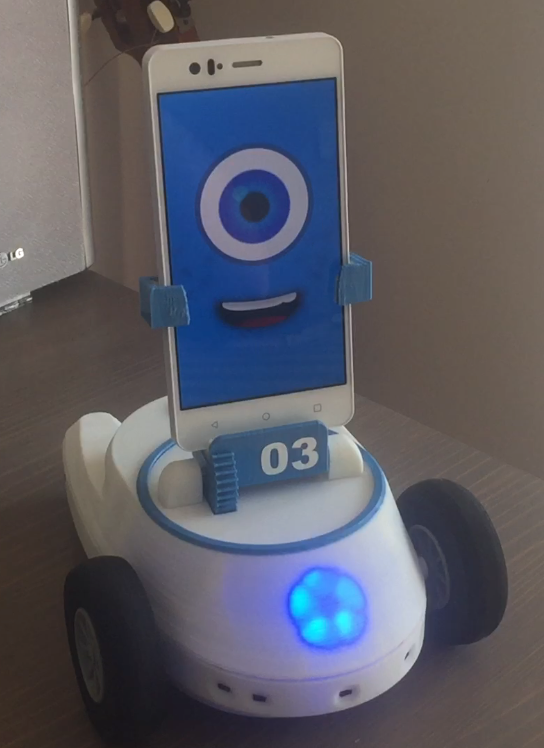
\includegraphics[width=1\linewidth]{imagenes/vigilante_standby.png}
\caption{ROBOBO en standby}
\label{fig:vigilante-standby}

\end{minipage}\hfill
\begin{minipage}{0.45\textwidth}
\centering
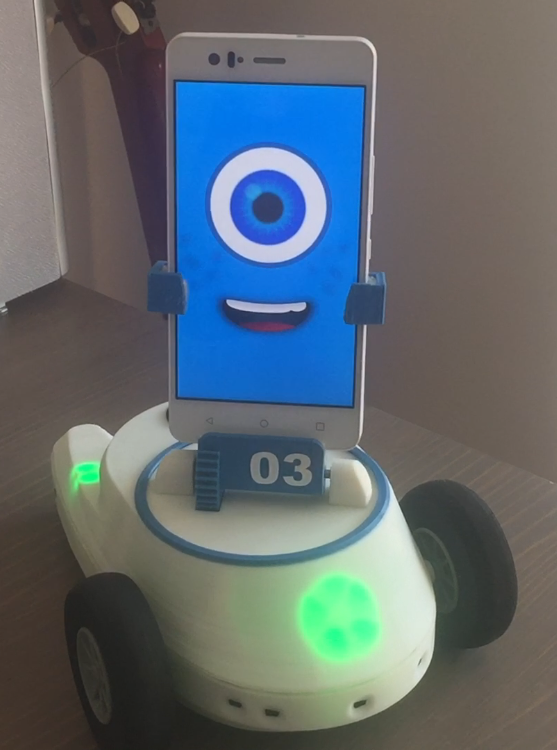
\includegraphics[width=1\linewidth]{imagenes/vigilante_patrol.png}

\caption{ROBOBO en modo patrulla}
\label{fig:vigilante-patrol}

\end{minipage}
\end{figure}

\begin{figure}
\centering
\begin{minipage}{0.45\textwidth}
\centering
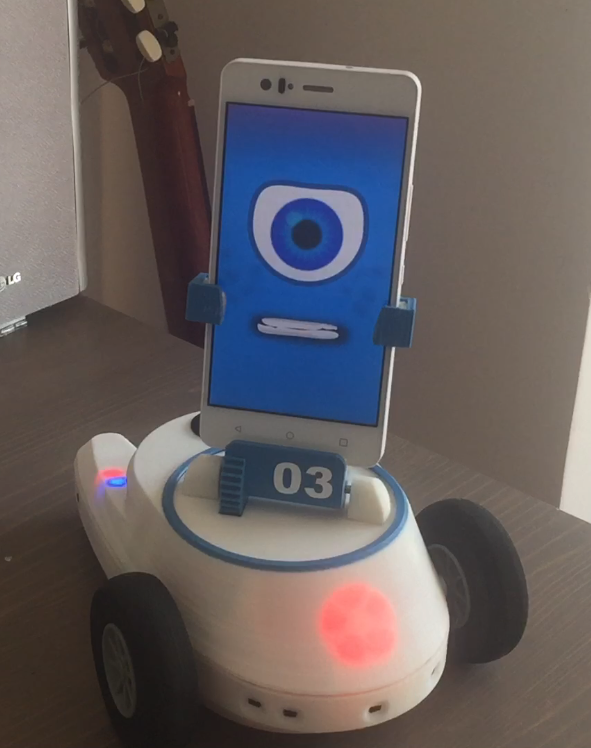
\includegraphics[width=1\linewidth]{imagenes/vigilante_alarm.png}
\caption{ROBOBO con la alarma activada}
\label{fig:vigilante-alarm}

\end{minipage}\hfill
\begin{minipage}{0.45\textwidth}
\centering
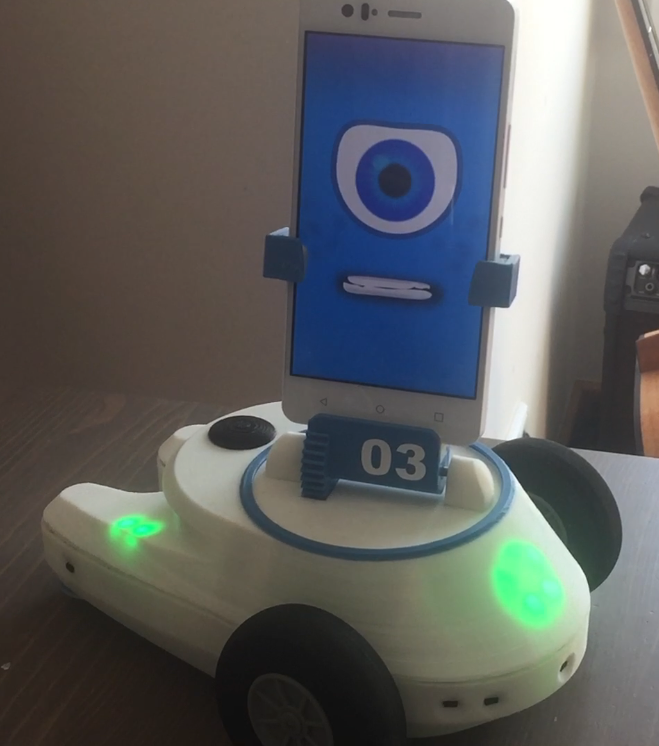
\includegraphics[width=1\linewidth]{imagenes/vigilante_silentmode_alarm.png}

\caption{ROBOBO con la alarma activada en modo silencioso}
\label{fig:vigilante-silentmode}

\end{minipage}
\end{figure}


\begin{figure}[h]
	\centering
	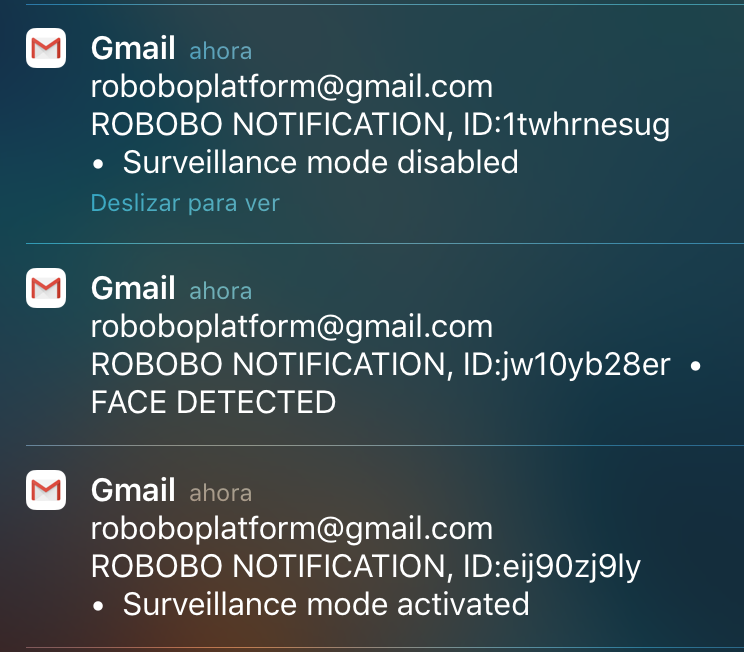
\includegraphics[width=0.6\linewidth]{imagenes/vigilante_mails.png}
	\caption{Mensajes enviados por el ROBOBO}
	\label{fig:vigilante-mails}
\end{figure} 



La gramática definida para este ejemplo es la siguiente:

\begin{verbatim}






#JSGF V1.0;
grammar voicecontrol;

<starter> = rob;
<activation> =activate|deactivate;
<mode>= face detection|sound detection|silent mode|movement;
<ending> = now;

<options> = <starter> switch <mode> <ending>;
<activations> = <starter> <activation> <ending>;

public <order> = <options>|<activations>;







\end{verbatim}


\begin{figure}
	\centering
	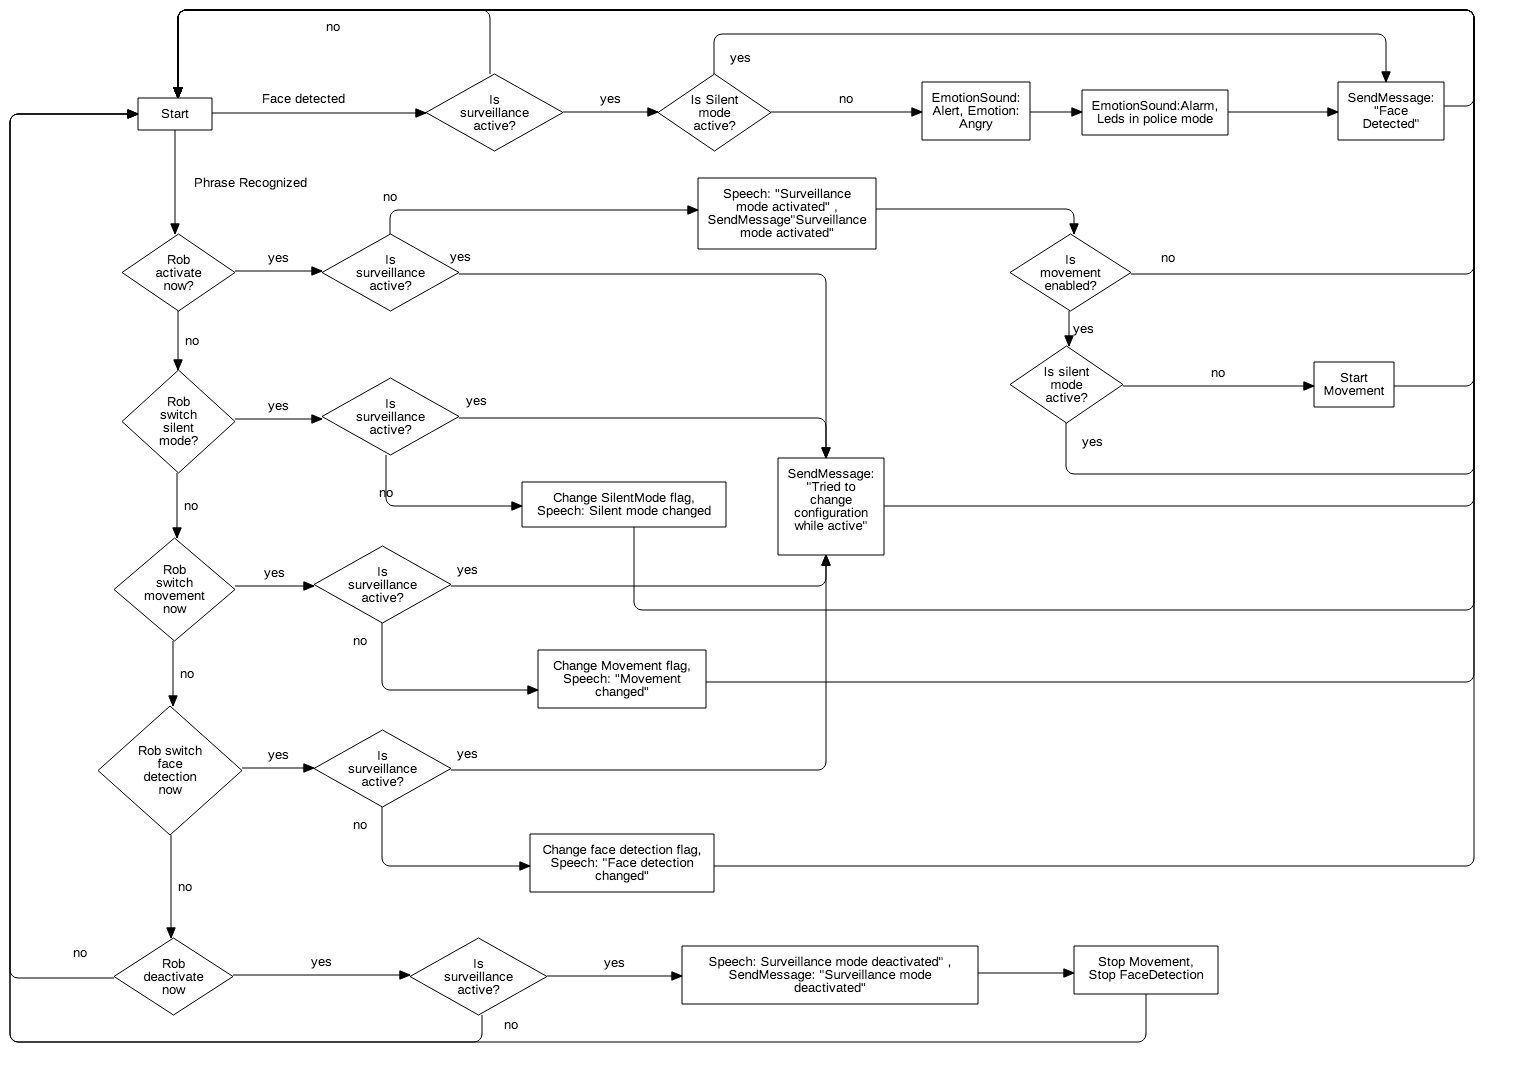
\includegraphics[width=1\linewidth]{imagenes/vigilante_diagram.png}
	\caption{Diagrama del flujo  ejecución del ejemplo de vigilancia}
	\label{fig:vigilante-diagram}
\end{figure} 

A continuación se puede ver un fragmento de código, la implementación del listener de detección de caras, en el cual se puede ver en funcionamiento el módulo de mensajería y el de sonidos prefijados:
\begin{lstlisting}
    @Override
    public void onFaceDetected(PointF faceCoords, float eyesDistance) {
        if (facedetection&&active) {
            if ((System.currentTimeMillis() - lastDetection) > 10000) {
                lastDetection = System.currentTimeMillis();
                if (!silentmode) {
                    policeTask = new PoliceTask();
                    policeTimer.scheduleAtFixedRate(policeTask, 2000, 200);
                    stopTimer.schedule(new StopTask(), 10000);
                    emotionSoundModule.playSound(IEmotionSoundModule.ALERT_SOUND);
                    alarmTimer.schedule(new AlarmTask(),1000);
                }
                emotionModule.setTemporalEmotion(Emotion.ANGRY, 10000, Emotion.NORMAL);
                msgModule.sendMessage("FACE DETECTED", "xxxxxxxxx@gmail.com", actualFrame.getBitmap());
            }
        }
    }
\end{lstlisting}
En el siguiente fragmento se puede observar un trozo del listener del módulo \textit{SpeechRecognition}, en el cual se muestra la detección de frases y el módulo de producción de habla en funcionamiento:
\begin{lstlisting}
	 @Override
    public void phraseRecognized(String phrase, Long timestamp) {
        String status = "";
        if (!active){
        if (phrase.equals("rob activate now")) {
            msgModule.sendMessage("Surveillance mode activated", "lfllamas93@gmail.com");

            active = true;
            speechProductionModule.sayText("Surveillance mode is now active",ISpeechProductionModule.PRIORITY_HIGH);
            startSurveillance();

        }

        if (phrase.equals("rob switch silent mode now")) {
            silentmode = !silentmode;
            if (silentmode){
                status = "active";
            }else{
                status = "disabled";
            }
            speechProductionModule.sayText("Silent mode is now "+status,ISpeechProductionModule.PRIORITY_HIGH);

        }
\end{lstlisting}


Este ejemplo no trata de ser un sistema de seguridad eficaz, sino demostrar una posible aplicación de los módulos desarrollados en este trabajo.

\newpage

%%%%%%%%%%%%%%%%%%%%%%%%%%%%%%%%%%%%%%%%%%%%%%%%%%%%%%%%%%
\subsection{ROBOBO Mascota}
\label{subsec:robobo-mascota}
Este este ejemplo, el ROBOBO interactuará a modo de mascota con el usuario, le pedirá que lo alimente, tratará de llamar la atención a su \enquote{cuidador} y reaccionará a sus acciones. 

En este ejemplo se han utilizado de forma conjunta la mayoría de los módulos desarrollados para permitir una interacción fluida con el robot. Los módulos empleados se presentan a continuación:




\begin{itemize}
	%\item SoundDispatcherModule: Necesario para el funcionamiento de los módulos de sonido
	%\item ClapDetectionModule: Se usa, con un umbral de detección sensible, para detectar sonidos en la zona.
	\item \textbf{EmotionSoundModule}: Diferentes sonidos son reproducidos en función de la interacción con el robot.
	\item \textbf{SpeechProductionModule}: Usado para transmitir las necesidades del robot al usuario.
	\item \textbf{SpeechRecognitionModule}: Usado para la comunicación por voz con el robot
	\item \textbf{BasicCameraModule}: Permite la captura de imágenes desde la cámara en segundo plano
	\item \textbf{FaceDetectionModule}: Permite la detección de caras y que el robot reaccione en función de su proximidad.
	\item \textbf{TouchModule}: Permite la interacción con el robot mediante gestos táctiles, por ejemplo acariciándolo o haciéndole cosquillas.
	\item \textbf{NoteProductionModule}: Permite al robot realizar secuencias de notas para llamar la atención al usuario.
	\item \textbf{ColorDetectionModule}: Permite la \enquote{alimentación} del robot mediante colores.
	\end{itemize}

Además de los módulos creados en este trabajo, se emplean varios módulos proporcionados por el ROBOBO! Framework:

\begin{itemize}
	\item \textbf{EmotionModule}: Provee la cara del robot, con la posibilidad de cambiar sus expresiones, es la interfaz gráfica que se le muestra al usuario.
	\item \textbf{DefaultMovementModule}: Permite el uso de la plataforma robótica de forma simple, permitiendo el movimiento del robot.
	\item \textbf{IRobInterfaceModule}: Proporciona un método para obtener la clase IRob, que se emplea para un control más avanzado del ROB, por ejemplo, para utilizar los leds de la base.
\end{itemize}


Este ejemplo no sigue un camino de ejecución definido como los ejemplos anteriores, sino que es guiado por la interacción con el usuario y una serie de eventos aleatorios, dichos eventos son los siguientes:

\begin{itemize}
	\item Movimientos: De vez en cuando el robot realizará diferentes movimientos, por ejemplo, girando sobre sí mismo, para llamar la atención del usuario.
	\item Caricias: A veces pedirá al usuario que lo acaricie.
	\item Hambre: Un contador de hambre irá disminuyendo a lo largo del tiempo, en el momento que baje de cierto umbral pedirá al usuario que lo alimente con un color determinado
	\item Sed: De manera semejante al hambre, un  contador de sed irá disminuyendo y en el caso de ser bajo, el usuario deberá darle de beber con el color azul.
	\item Silbidos: Para llamar la atención del usuario el robot hará sonar una melodía aleatoria a modo de silbido.
\end{itemize}

La interacción mediante caras depende de la distancia a la que se encuentre el usuario, si está demasiado cerca, el ROBOBO tendrá verguenza y se alejará(figura \ref{fig:pet_close}), sin embargo si considera que el usuario esta muy lejos le dirá que se acerque. Si además cuando detecte una cara es la primera detección, saludará al usuario y se presentará.

El siguiente fragmento de código es la implementación del listener del detector de caras, empleado para saber la distancia del usuario al robot:

\begin{lstlisting}
	//region FaceListener
    @Override
    public void onFaceDetected(PointF faceCoords, float eyesDistance) {
        Log.d(TAG,"Eyes distance: "+eyesDistance);
        if (eyesDistance>150){
            emotionModule.setTemporalEmotion(Emotion.EMBARRASED,2000,Emotion.NORMAL);
            speechModule.sayText("You are too close!",ISpeechProductionModule.PRIORITY_LOW);
            try {
                movementModule.moveBackwardsTime((short)20,2000);

            } catch (InternalErrorException e) {
                e.printStackTrace();
            }
        }else if (eyesDistance<50){
            emotionModule.setTemporalEmotion(Emotion.SURPRISED,2000,Emotion.NORMAL);
            speechModule.sayText("You are too far! Come here!",ISpeechProductionModule.PRIORITY_LOW);
            
        }else{
            if (firstface){
                firstface = false;
                emotionModule.setTemporalEmotion(Emotion.HAPPY,5000,Emotion.NORMAL);
                speechModule.sayText("Hey there! Im robobo!", ISpeechProductionModule.PRIORITY_HIGH);

            }
        }
    }
    //endregion
\end{lstlisting}


\begin{figure}
\centering
\begin{minipage}{0.45\textwidth}
\centering
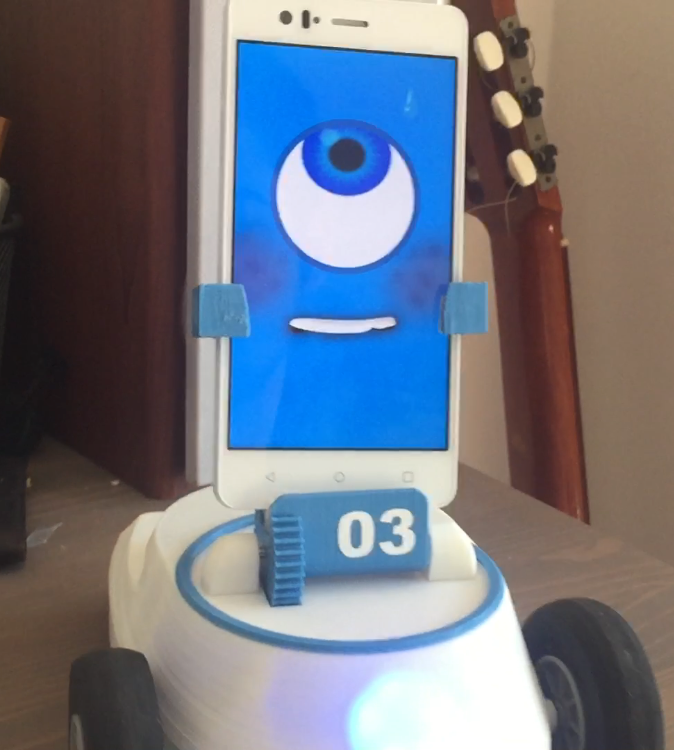
\includegraphics[width=1\linewidth]{imagenes/pet_close.png}
\caption{ROBOBO retrocediendo de una cara cercana}
\label{fig:pet_close}

\end{minipage}\hfill
\begin{minipage}{0.45\textwidth}
\centering
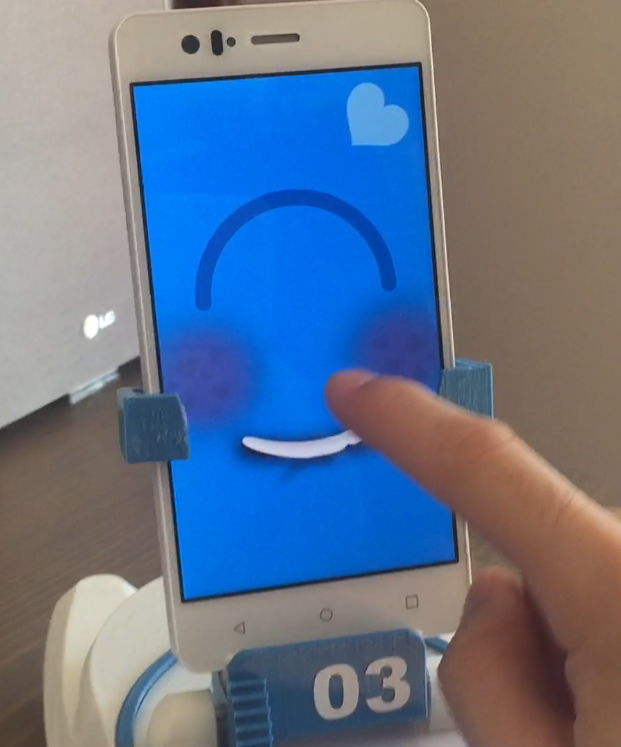
\includegraphics[width=1\linewidth]{imagenes/pet_pet.png}

\caption{ROBOBO ante caricias}
\label{fig:pet_pet}

\end{minipage}
\end{figure}

\begin{figure}
\centering
\begin{minipage}{0.45\textwidth}
\centering
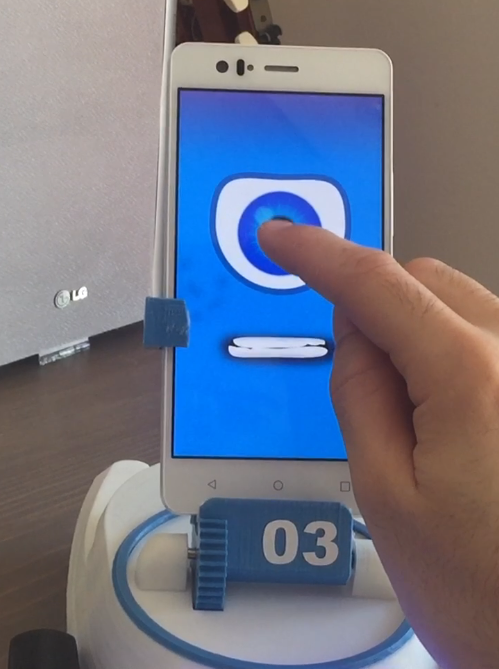
\includegraphics[width=1\linewidth]{imagenes/pet_eye.png}
\caption{ROBOBO tras tocarle el ojo}
\label{fig:pet_eye}

\end{minipage}\hfill
\begin{minipage}{0.45\textwidth}
\centering
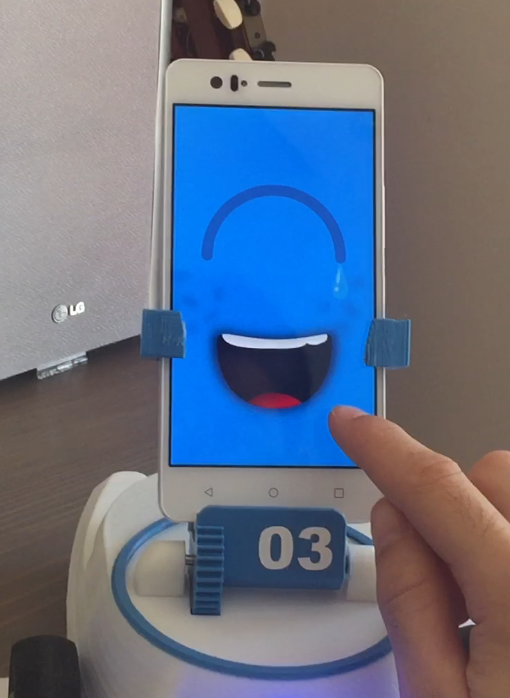
\includegraphics[width=1\linewidth]{imagenes/pet_tickles.png}

\caption{ROBOBO con cosquillas}
\label{fig:pet_tickles}

\end{minipage}
\end{figure}






La interacción táctil es diferente según el gesto que se realice:
\begin{itemize}
	\item Tap: dependiendo de donde sea el toque reaccionará de forma distinta
	\begin{itemize}
		\item Ojo: Se quejará por meterle el dedo en el ojo y retrocederá un poco(figura \ref{fig:pet_eye})
		\item Boca: Reaccionará de manera similar a con el ojo
		\item Resto del la pantalla: Pondrá cara de risa y dirá que tiene cosquillas (figura \ref{fig:pet_tickles})
	\end{itemize}
	\item Fling: Ejecutará diferentes movimientos en función de la dirección del fling
	\item Touch: El tilt del ROB volverá a su posición original
	\item Caress: Solo reaccionará si ha pedido previamente una caricia, agradeciéndoselo al usuario(figura \ref{fig:pet_pet}).
\end{itemize}

A continuación se ve la implementación del listener del tap:
\begin{lstlisting}
	@Override
    public void tap(Integer x, Integer y) {
        Log.d(TAG,"X: "+x+" Y: "+y);
        if ((x>230)&&(x<900)&&(y>425)&&(y<1025)){
            emotionModule.setTemporalEmotion(Emotion.ANGRY,2000,Emotion.NORMAL);
            speechModule.sayText("Ouch! Don't poke my eye!",ISpeechProductionModule.PRIORITY_HIGH);

        }else if ((x>250)&&(x<800)&&(y>1285)&&(y<1500)){
            emotionModule.setTemporalEmotion(Emotion.ANGRY,2000,Emotion.NORMAL);
            speechModule.sayText("Dont put your finger in my mouth!",ISpeechProductionModule.PRIORITY_HIGH);

        }else{
            emotionModule.setTemporalEmotion(Emotion.LAUGHING,2000,Emotion.NORMAL);
            speechModule.sayText("That tickles!",ISpeechProductionModule.PRIORITY_HIGH);
        }
    }
\end{lstlisting}

La interacción por voz se usa para comunicar al robot diferentes cosas:
\begin{itemize}
	\item \textit{Here comes the food}: Prepara al robot para recibir comida en forma de color
	\item \textit{Here comes the drink}: Prepara al robot para recibir bebida en forma de color.
	\item \textit{Hello}: Saluda al robot, que responderá al saludo.
	\item \textit{How are you}: Pregunta al robot su estado, que responderá con sus niveles de hambre y sed.
	\item \textit{Do a trick}: Pide al robot que realice un truco.
\end{itemize}

El módulo de detección de colores solo será activado después de que el usuario manifieste su intención, mediante voz, de alimentar o dar de beber al robot.
Si el color mostrado al robot es el adecuado, este dará las gracias y el contador de comida/agua será restablecido al máximo. En caso de fallar el color, el robot se quejará y continuará la detección de colores.


A continuación se muestra la implementación del listener de colores para alimentar al ROBOBO:
\begin{lstlisting}
	//region ColorListener
    @Override
    public void onNewColor(int colorrgb, int nearest_color) {
        if (expectedColor == nearest_color){
            speechModule.sayText("Thank You!", ISpeechProductionModule.PRIORITY_LOW);
            if ((expectedColor == android.graphics.Color.GREEN)||(expectedColor == android.graphics.Color.RED)){
                foodlevel=5;
            }else{
                waterlevel= 5;
            }
            colorDetectionModule.pauseDetection();
        }else{
            speechModule.sayText("I didnt ask for this!", ISpeechProductionModule.PRIORITY_LOW);
        }
    }
    //endregion
\end{lstlisting}


\section{Resultados de los ejemplos}
\label{sec:example-results}

Los tres ejemplos fueron probados y respondieron de la manera esperada, sin embargo, como en todo proyecto de HRI, el ajuste es una parte importante del desarrollo y la experiencia de interacción mejorará según el sistema sea usado por diversos usuarios y se reciba información por parte de los mismos que permita un ajuste fino de las librerías desarrolladas.





%%%%%%%%%%%%%%%%%%%%%%%%%%%%%%%%%%%%%%%%%%%%%%%%%%%%%%%%%
\newpage
\section{Problemas conocidos}
\begin{itemize}
	\item La tasa de refresco del módulo \textit{BasicCamera} es baja y varía mucho entre terminales móviles.
	\item El \textit{ColorDetectionModule} puede confundirse si el fondo no es homogéneo, se recomienda usar tarjetas con colores sobre fondo blanco.
	\item El \textit{EmailModule} puede causar el bloqueo de la cuenta de Gmail si esta no es configurada previamente para usar mediante IMAP.
	\item El \textit{TouchModule} requiere el paso explícito de los TouchEvents de la actividad en pantalla.
	\item El sistema Android no permite el uso del micrófono por más de un thread al mismo tiempo, lo que hace que los módulos que usan el micrófono de la librería Sound sean incompatibles con el módulo \textit{SpeechRecognition}.
\end{itemize}
\label{sec:known_issues}
    

